\documentclass[../main/thesis.tex]{subfiles}
\begin{document}
%\appendixpagenumbering
%\chapter{Appendix}
%\addcontentsline{toc}{chapter}{Appendix}
%\appendixpagenumbering
%\appendix
%\section{PCB for detector connection}
%\appendixpagenumbering
A \gls{PCB} was needed to connect the detector to the outside world, as the detector pads are too small for any other connection than wire-bonding. This \gls{PCB} could simply have consisted of wire-bonding pads going to connectors for cables, but it was decided to make a more multi-purpose board to make it simple to try different set-ups. The board was made so that it is possible to connect the substrate, the guard rings, and the p+ rings individually to ground or external bias. It is also possible to read out the guard rings of the cells. Each channel can also be connected to a bias filter for removal of high frequency noise. The n+ core readout channel was designed to add as little capacitance as possible. LEMO connectors were chosen to connect to the outside world as they are well shielded and much used at \gls{ift}. The exposed metal is coated with electroless nickel immersion gold (ENIG) to provide better contact for wire-bonding. The layout of the \gls{PCB} can be seen in figure \ref{fig-pcb} and a photograph can be seen in figure \ref{fig-pcb-pic}. 

\begin{figure}%[h]
	\centering
	%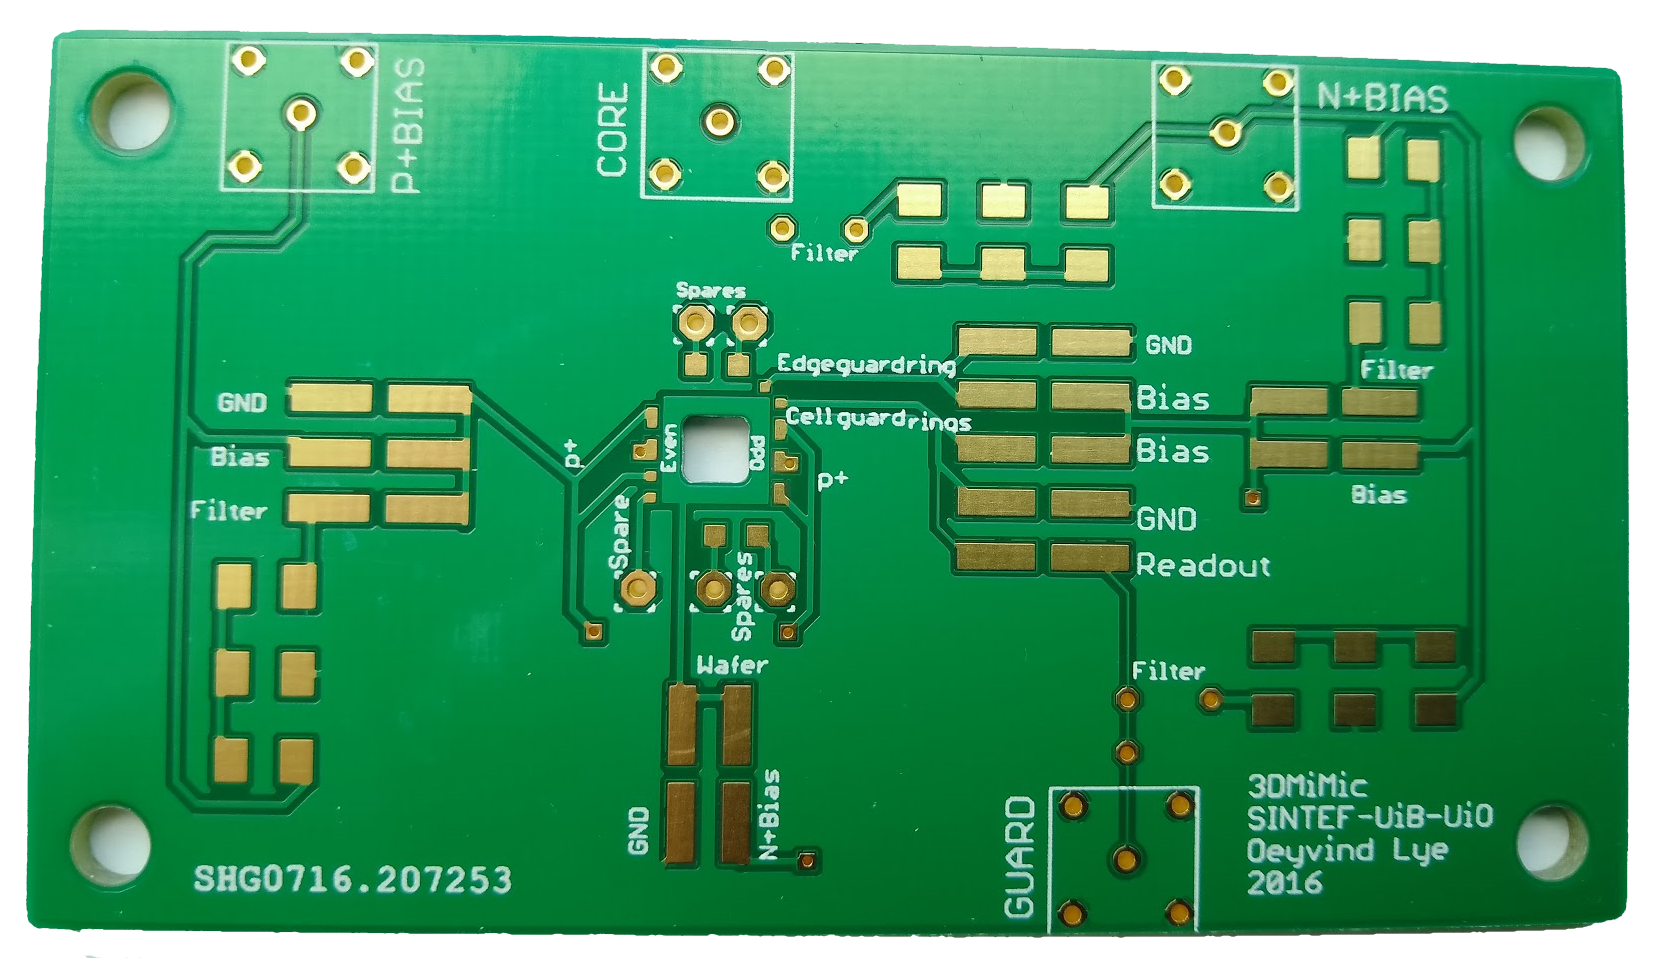
\includegraphics[angle=270,\textwidth]{pcb-pic.png}
	\caption{Top side of PCB.}
	\label{fig-pcb-pic} 
\end{figure}

\begin{figure}%[h]
	\centering
	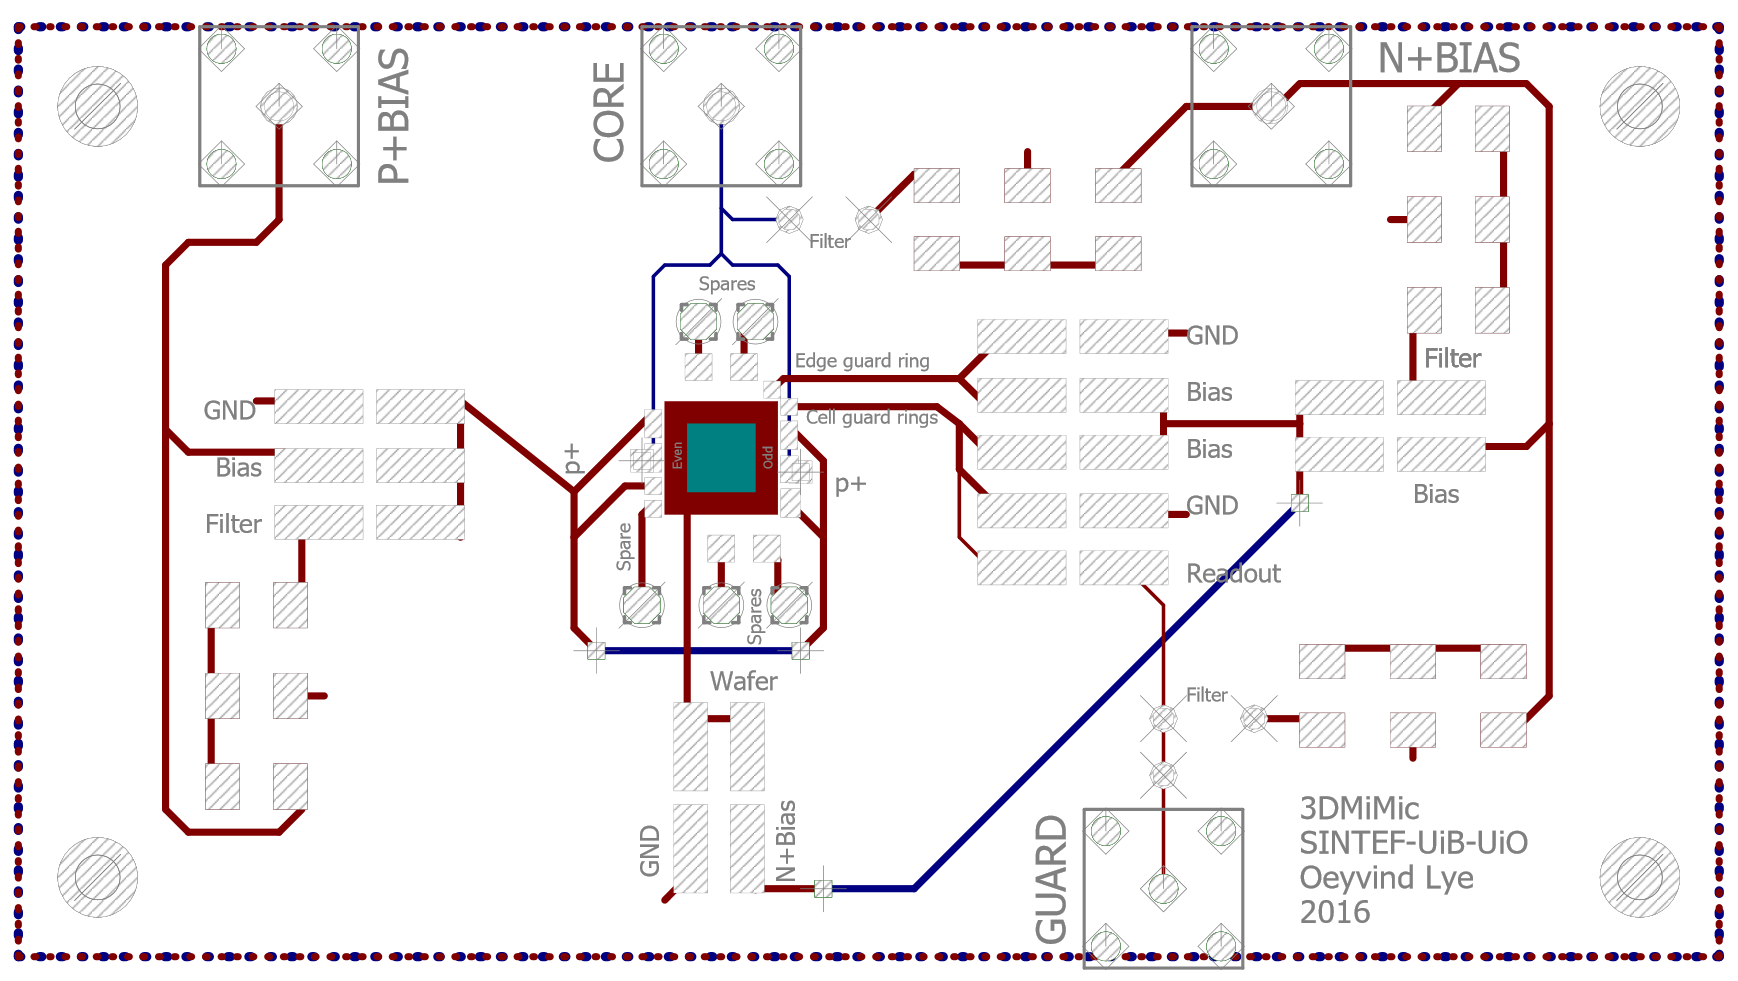
\includegraphics[angle=270,width=0.8\textwidth]{pcb.png}
	\caption{PCB layout. Ground planes not shown.}
	\label{fig-pcb} 
\end{figure}


\end{document}